\documentclass[../main.tex]{subfiles}

\begin{document}
\section{UCB-BAR: Rocket Chip Generator}
\begin{figure}
    \centering
    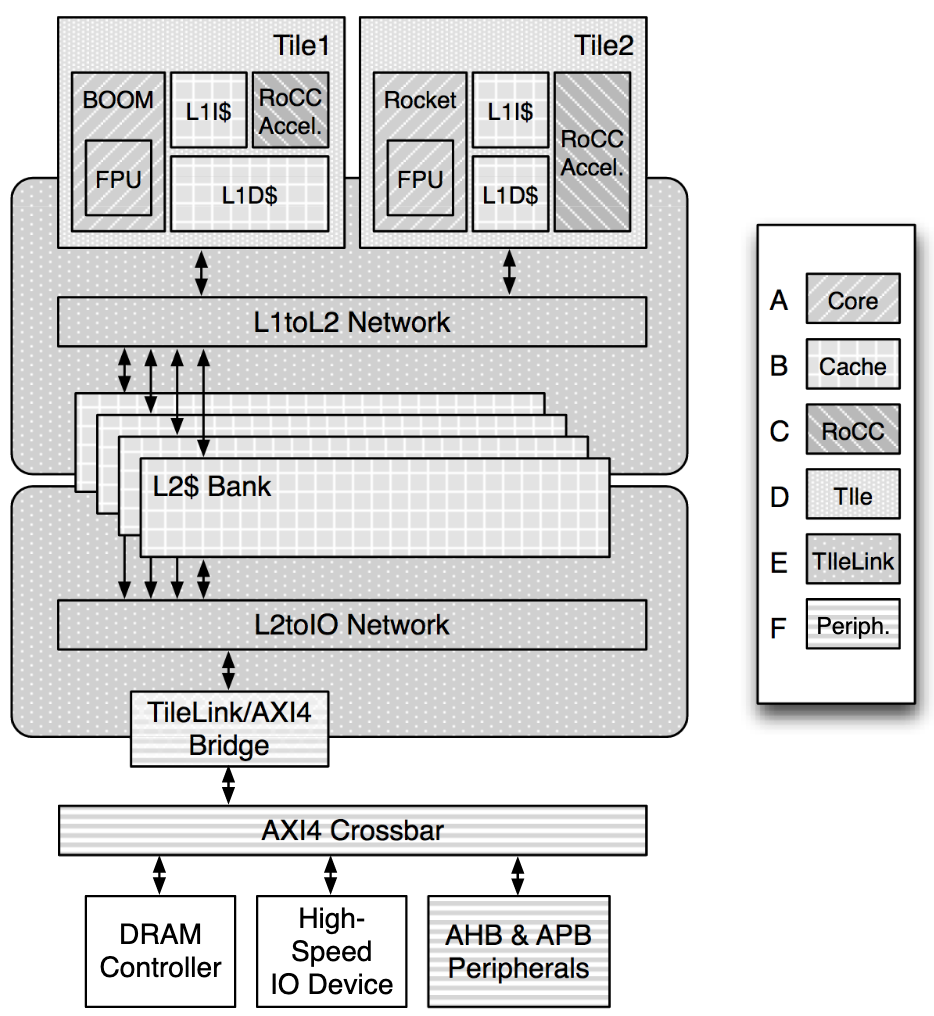
\includegraphics[scale=.4]{pngs/RocketChipGeneratorLayout.png}
    \caption{Rocket Chkp Pipeline\cite{Asanović:EECS-2016-17}}
    \label{fig:RocketCipGen}
\end{figure}
The University of California, Berkeley (UCB) developed the Rocket chip Generator, and the Chips Alliance foundation maintains this generator\cite{Chips-Alliance}. It generates a SOC with caches and tiles, process sub-modules. This section covers the default chiplet created by the generator; see figure \ref{fig:RocketCipGen} for an overview of the default chiplet.

\subsection{Generic Rocket Chip}
This sub-section gives an overview of the modules in the default Rocket chiplet. The lowes layer is the tile layer. This layer is where the processor,  L1 instruction, and L2 Data cache reside. In addition to these modules, a tile can instantiate a rocket custom co-processor (RoCC).  The tile defaults to one of the following cores: Rocket core, or Berkeley out of order machine (BOOM) core. Any processor that can interface with the system can substitute the place of the two core mentioned prior.  The default RoCC is a basic multiply accumulator unit. One of the notable RoCC is the Hwacha Vector-Fetch co-processor\cite{HwachaPaper}. The next layer is the L2 caches layer. These two layers connect through the L1ToL2 tile link bus. The top layer is the IO layer, and it connects through L2ToIO tile link bus. The Rocket chiplet's IO consist of one advanced extensible interface (AXI) bus and one host bus, direct memory interface (DMI). 



\subsection{Rocket Core}
\begin{figure}
    \centering
    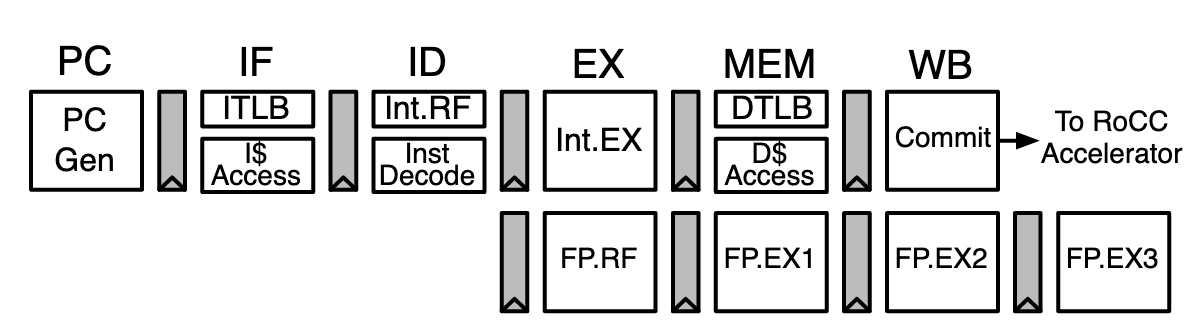
\includegraphics[scale=.4]{pngs/RocketPipeline.png}
    \caption{Rocket Chkp Pipeline\cite{Asanović:EECS-2016-17}}
    \label{fig:RocketCipFlow}
\end{figure}
This sub-section details the RISC-V based Rocket core. This core is a single fetch, single issue, in-order scalar processor, and figure \ref{fig:RocketCipFlow} shows the pipeline for this processor. Rocket core supports the IMAFG instruction set architecture (ISA) extensions\cite{RISC-V-isa}. IMAFG extensions represent the following functionality: integer (I), multiply and divide (M), atomic (A), single-precision (F), and double-precision (D) floating-point\cite{RISC-V-isa}. In addition to the IMAFG extension, this core supports the E extension. E extension stands for the custom extension. This extension is used to communicate with the RoCC unit.


\subsection{Chisel}
The Rocket chip generator uses the hardware construction language (HCL) Chisel\cite{chisel:book}. Chisel embeds itself into the Scala programming language. Because Chisel builds upon Scala, it gains a high-level of abstraction. With the ability to create a high level of abstraction, sophisticated hardware designs become more simplistic to design. The goal of Chisel is to merge hardware development with software development\cite{chisel:book}. Most low-level hardware description languages (HDL) cannot generate sophisticated hardware based on complex functions. Chisel allows the use of functions to drive the hardware generation\cite{chisel:book}.


\subsection{Configuring the Rocket Chip Generator}
The Rocket chip generator contains many different generators. Most complex modules in Chisel contain a generator or two. At the top-level, a generator consumes a set of configuration and passes it down to each module in its hierarchy. Sets of configuration can be combined to create a complex set of configurations. Figure \ref{fig:configsnipit} shows how to add a RoCC unit to a default Rocket core. 

\begin{figure}
    \centering
    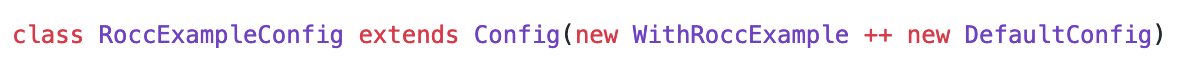
\includegraphics[scale=.4]{pngs/ConfigSnipit.png}
    \caption{ROCC Example Config}
    \label{fig:configsnipit}
\end{figure}
\end{document}